% Preámbulo
\documentclass[letterpaper]{article}
\usepackage[utf8]{inputenc}
\usepackage[spanish]{babel}

\usepackage{enumitem}
\usepackage{titling}

% Símbolos
	\usepackage{amsmath}
	\usepackage{amssymb}

% Márgenes
	\usepackage
	[
		margin = 1.23in
	]
	{geometry}

% Imágenes
	\usepackage{float}
	\usepackage{graphicx}
	\graphicspath{{Images/}}
	\usepackage{subcaption}

% Ambientes
	\usepackage{amsthm}

	\renewcommand{\qedsymbol}{$\blacksquare$}

	\theoremstyle{definition}
	\newtheorem{ejercicio}{Ejercicio}

	\newtheoremstyle{lemathm}{4pt}{0pt}{\itshape}{0pt}{\bfseries}{ --}{ }{\thmname{#1}\thmnumber{ #2}\thmnote{ (#3)}}
	\theoremstyle{lemathm}
	\newtheorem{lema}{Lema}

	\newtheoremstyle{lemademthm}{0pt}{10pt}{\itshape}{ }{\mdseries}{ --}{ }{\thmname{#1}\thmnumber{ #2}\thmnote{ (#3)}}
	\theoremstyle{lemademthm}
	\newtheorem*{lemadem}{Demostración}

% Ajustes
	\allowdisplaybreaks	% Los align pueden cambiar de página

% Macros
	\newcommand{\sumi}[2]{\sum_{i=#1}^{#2}}
	\newcommand{\dint}[2]{\displaystyle\int_{#1}^{#2}}
	\newcommand{\inte}[2]{\int_{#1}^{#2}}
	\newcommand{\dlim}{\displaystyle\lim}
	\newcommand{\limxinf}{\lim_{x\to\infty}}
	\newcommand{\limninf}{\lim_{n\to\infty}}
	\newcommand{\dlimninf}{\displaystyle\lim_{n\to\infty}}
	\newcommand{\limh}{\lim_{h\to0}}
	\newcommand{\ddx}{\dfrac{d}{dx}}
	\newcommand{\txty}{\text{ y }}
	\newcommand{\txto}{\text{ o }}
	\newcommand{\Txty}{\quad\text{y}\quad}
	\newcommand{\Txto}{\quad\text{o}\quad}
	\newcommand{\si}{\text{si}\quad}
	\newcommand{\abs}[1]{\left| #1 \right| }
	\newcommand{\bars}[1]{\left \| #1 \right \| }
	\newcommand{\pars}[1]{\left( #1 \right) }
	\newcommand{\bracs}[1]{\left[ #1 \right] }
	\newcommand{\floor}[1]{\left \lfloor #1 \right\rfloor }
	\newcommand{\ceil}[1]{\left \lceil #1 \right\rceil }
	\newcommand{\angles}[1]{\left \langle #1 \right\rangle }
	\newcommand{\set}[1]{\left \{ #1 \right\} }
	\newcommand{\norma}[2]{\left\| #1 \right\|_{#2} }

	\newcommand{\etiqueta}{\stepcounter{equation}\tag{\theequation}}
	\newcommand{\tq}{:}
	\renewcommand{\o}{\circ}
	% \newcommand*{\QES}{\hfill\ensuremath{\boxplus}}
	% \newcommand*{\qes}{\hfill\ensuremath{\boxminus}}
	% \newcommand*{\qeshere}{\tag*{$\boxminus$}}
	% \newcommand*{\QESHERE}{\tag*{$\boxplus$}}
	\newcommand*{\QES}{\hfill\ensuremath{\blacksquare}}
	\newcommand*{\qes}{\hfill\ensuremath{\square}}
	\newcommand*{\QESHERE}{\tag*{$\blacksquare$}}
	\newcommand*{\qeshere}{\tag*{$\square$}}
	\newcommand*{\QED}{\hfill\ensuremath{\blacksquare}}
	\newcommand*{\QEDHERE}{\tag*{$\blacksquare$}}
	\newcommand*{\qel}{\hfill\ensuremath{\boxdot}}
	\newcommand*{\qelhere}{\tag*{$\boxdot$}}
	\renewcommand*{\qedhere}{\tag*{$\square$}}

	\newcommand{\suc}[1]{\left(#1_n\right)_{n\in\N}}
	\newcommand{\en}[2]{\binom{#1}{#2}}
	\newcommand{\upsum}[2]{U(#1,#2)}
	\newcommand{\lowsum}[2]{L(#1,#2)}

	\newcommand{\N}{\mathbb{N}}
	\newcommand{\Q}{\mathbb{Q}}
	\newcommand{\R}{\mathbb{R}}
	\newcommand{\Z}{\mathbb{Z}}
	\newcommand{\eps}{\varepsilon}
	\newcommand{\ttF}{\mathtt{F}}
	\newcommand{\bfF}{\mathbf{F}}

	\newcommand{\To}{\longrightarrow}
	\newcommand{\mTo}{\longmapsto}
	\newcommand{\ssi}{\Longleftrightarrow}
	\newcommand{\sii}{\Leftrightarrow}
	\newcommand{\then}{\Rightarrow}

	\newcommand{\pTFC}{{\itshape 1er TFC\/}}
	\newcommand{\sTFC}{{\itshape 2do TFC\/}}
    
% Datos
    \title{Álgebra para Ciencias de la Computación\\Examen Parcial I}
    \author{Rubén Pérez Palacios\\Profesor: Dr. Rafael Herrera Guzmán}
    \date{11 de Septiembre 2020}

% DOCUMENTO
\begin{document}
	\maketitle
    
    \section*{Problemas}

    \begin{enumerate}
		
		\item Sean $a=(1,2,1)$, $b=(0,4,5)$, $c=(-1,0,7)$. Calcula
		
		\[a \wedge b, \quad b \wedge c, \quad a \wedge b \wedge c\]

		en términos de los vectores básicos $e_1,e_2,e_3 \in \R^3$ y describe la interpretación geométrica de los distintos coeficientes.

		Calculemos los bivectores y el trivector deseado.

		\begin{align*}
			a \wedge b &= (e_1 + 2e_2 + e_3) \wedge (4e_2 + 5e_3) & \text{Por base canónica}\\
			&= 4 e_1 \wedge e_2 + 8 e_2 \wedge e_2 + 4 e_3 \wedge e_2 + 5 e_1 \wedge e_3 + 10 e_2 \wedge e_3 + 5 e_3 \wedge e_3 & \text{Por distribución}\\
			&= 4 e_1 \wedge e_2 + 4 e_3 \wedge e_2 + 5 e_1 \wedge e_3 + 10 e_2 \wedge e_3 & \text{Por $x \wedge x = 0$}\\
			&= 4 e_1 \wedge e_2 + 5 e_1 \wedge e_3 + 6 e_2 \wedge e_3 & \text{Por antisimetría}\\
			b \wedge c &= (4e_2 + 5e_3) \wedge (-e_1 + 7e_3) & \text{Por base canónica}\\
			&= -4 e_2 \wedge e_1 - 5 e_3 \wedge e_1 + 28 e_2 \wedge e_3 + 35 e_3 \wedge e_3 & \text{Por distribución}\\
			&= -4 e_2 \wedge e_1 - 5 e_3 \wedge e_1 + 28 e_2 \wedge e_3 & \text{Por $x \wedge x = 0$}\\
			&= 4 e_1 \wedge e_2 + 5 e_1 \wedge e_3 + 28 e_2 \wedge e_3 & \text{Por antisimetría}\\
			a \wedge b \wedge c &= (a \wedge b) \wedge c & \text{Por asociatividad}\\
			&= (4 e_1 \wedge e_2 + 5 e_1 \wedge e_3 + 6 e_2 \wedge e_3) \wedge (-e_1 + 7e_3) & \text{Por base canónica}\\
			&= -4 e_1 \wedge e_2 \wedge e_1 - 5 e_1 \wedge e_3 \wedge e_1 - 6 e_2 \wedge e_3 \wedge e_1 + 28 e_1 \wedge e_2 \wedge e_3\\
			& + 35 e_1 \wedge e_3 \wedge e_3 + 42 e_2 \wedge e_3 \wedge e_3 & \text{Por distribución}\\
			&= - 6 e_2 \wedge e_3 \wedge e_1 + 28 e_1 \wedge e_2 \wedge e_3 & \text{Por $x \wedge x = 0$}\\
			&= 22 e_1 \wedge e_2 \wedge e_3 & \text{Por antisimetría}\\
		\end{align*}

		\newpage

		Ahora veamos cuales son sus graficas asociadas y que orientación tienen.

		\begin{figure}[H]
			\begin{center}
				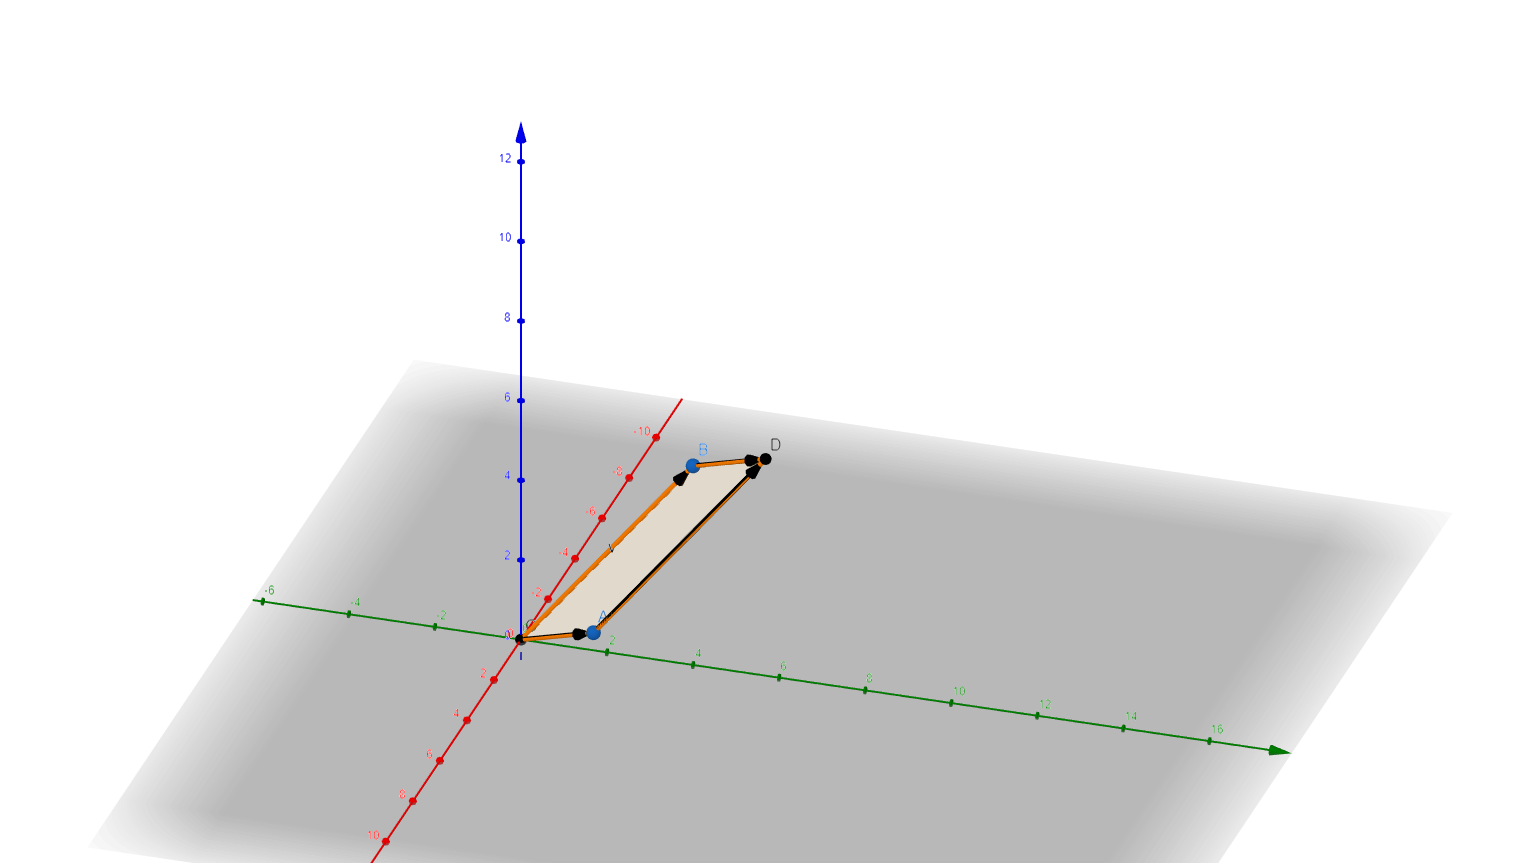
\includegraphics[scale=.17]{a^b.png}
				\caption*{$a \wedge b$, orientación de $\vec{a}$ al $\vec{b}$}
			\end{center}
		\end{figure}

		\begin{figure}[H]
			\begin{center}
				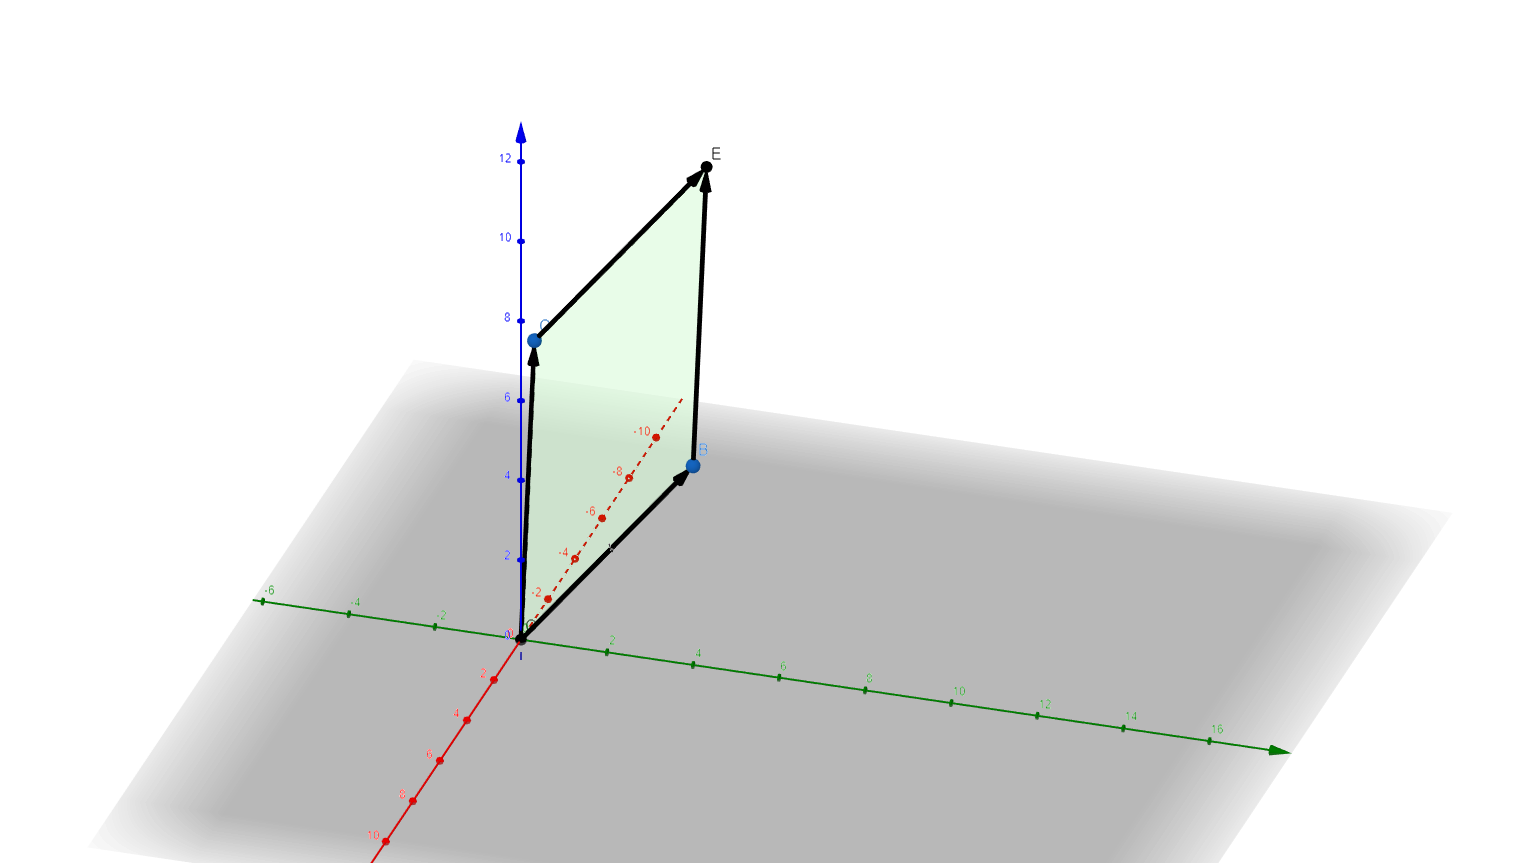
\includegraphics[scale=.17]{b^c.png}
				\caption*{$b \wedge c$, orientación de $\vec{b}$ al $\vec{c}$}
			\end{center}
		\end{figure}

		\begin{figure}[H]
			\begin{center}
				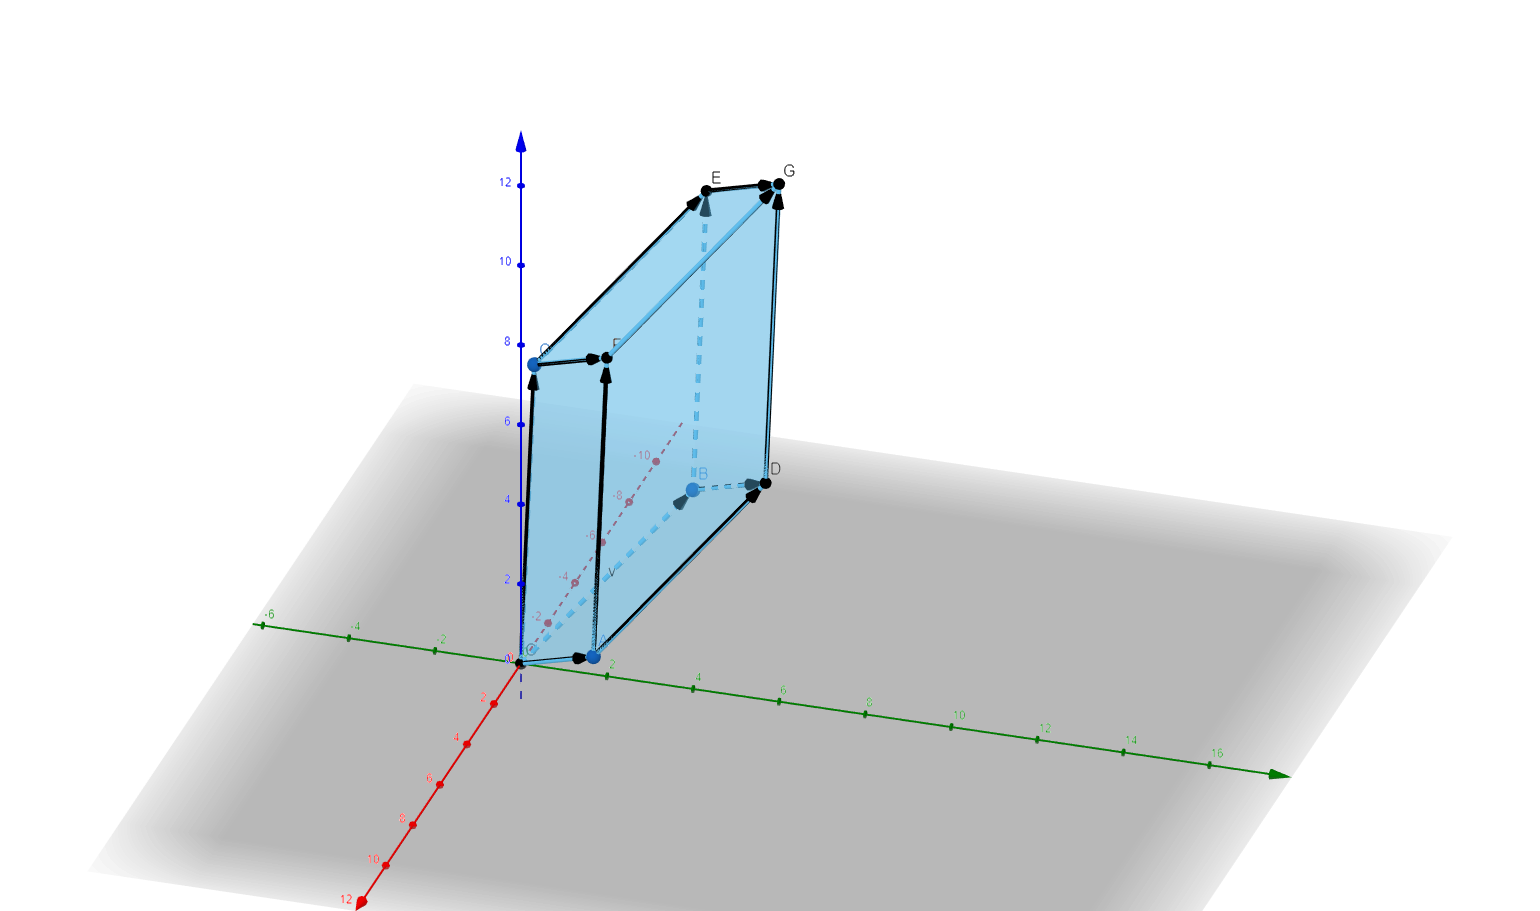
\includegraphics[scale=.17]{a^b^c.png}
				\caption*{$a \wedge b \wedge c$, forman un sitema de la mano derecha la cual es su horientación}
			\end{center}
		\end{figure}
		
		\newpage

		\item Calcula los determinantes, las adjuntas clásicas y, en caso de que exitan, la inversas de las siguientes matrices:
		
		\[A = \begin{pmatrix}
			6 & -1\\[1ex]
			2 & 3
		\end{pmatrix}, \quad B = \begin{pmatrix}
			1 & 0 & 4\\[1ex]
			0 & -1 & 3\\[1ex]
			2 & 0 & -5
		\end{pmatrix}.\]

		Los determinantes son

		\[\det(A) = 20, \quad \det(B) = 13.\]

		Las matrices adjuntas clásicas son

		\[\text{adj}(A) = C^T = \begin{pmatrix}
			3 & 1\\[1ex]
			-2 & 6
		\end{pmatrix}, \quad \text{adj}(B) = C^T = \begin{pmatrix}
			5 & 0 & 4\\[1ex]
			6 & -13 & -3\\[1ex]
			2 & 0 & -1
		\end{pmatrix}.\]

		Las matrices inversas son

		\[A^{-1} = \frac{\text{adj}(A)}{\det(B)} =  \begin{pmatrix}
			\frac{3}{20} & \frac{1}{20}\\[1ex]
			-\frac{1}{10} & \frac{3}{10}
		\end{pmatrix}, \quad B^{-1} = \frac{\text{adj}(B)}{\det(B)} = \begin{pmatrix}
			\frac{5}{13} & 0 & \frac{4}{13}\\[1ex]
			\frac{6}{13} & -1 & -\frac{3}{13}\\[1ex]
			\frac{2}{13} & 0 & -\frac{1}{13}
		\end{pmatrix}.\]

		\item Utilizando la matriz b del ejercicio anterior, calcula la matriz inducida en ${\bigwedge}^2\R^3$ con respecto a una base de bivectores de tu elección.
		
		La matriz inducida en ${\bigwedge}^2\R^3$ por $B$ con respecto a la base canónica es

		\[{\bigwedge}^2B = \begin{pmatrix}
			M_{33} & M_{32} & M_{31}\\[1ex]
			M_{23} & M_{22} & M_{21}\\[1ex]
			M_{13} & M_{12} & M_{11}
		\end{pmatrix} = \begin{pmatrix}
			-1 & 3 & 4\\[1ex]
			0 & -13 & 0\\[1ex]
			2 & -6 & 5
		\end{pmatrix}\]

	\end{enumerate}

	
\end{document}
